% Options for packages loaded elsewhere
\PassOptionsToPackage{unicode}{hyperref}
\PassOptionsToPackage{hyphens}{url}
%
\documentclass[
]{book}
\usepackage{amsmath,amssymb}
\usepackage{iftex}
\ifPDFTeX
  \usepackage[T1]{fontenc}
  \usepackage[utf8]{inputenc}
  \usepackage{textcomp} % provide euro and other symbols
\else % if luatex or xetex
  \usepackage{unicode-math} % this also loads fontspec
  \defaultfontfeatures{Scale=MatchLowercase}
  \defaultfontfeatures[\rmfamily]{Ligatures=TeX,Scale=1}
\fi
\usepackage{lmodern}
\ifPDFTeX\else
  % xetex/luatex font selection
\fi
% Use upquote if available, for straight quotes in verbatim environments
\IfFileExists{upquote.sty}{\usepackage{upquote}}{}
\IfFileExists{microtype.sty}{% use microtype if available
  \usepackage[]{microtype}
  \UseMicrotypeSet[protrusion]{basicmath} % disable protrusion for tt fonts
}{}
\makeatletter
\@ifundefined{KOMAClassName}{% if non-KOMA class
  \IfFileExists{parskip.sty}{%
    \usepackage{parskip}
  }{% else
    \setlength{\parindent}{0pt}
    \setlength{\parskip}{6pt plus 2pt minus 1pt}}
}{% if KOMA class
  \KOMAoptions{parskip=half}}
\makeatother
\usepackage{xcolor}
\usepackage{longtable,booktabs,array}
\usepackage{calc} % for calculating minipage widths
% Correct order of tables after \paragraph or \subparagraph
\usepackage{etoolbox}
\makeatletter
\patchcmd\longtable{\par}{\if@noskipsec\mbox{}\fi\par}{}{}
\makeatother
% Allow footnotes in longtable head/foot
\IfFileExists{footnotehyper.sty}{\usepackage{footnotehyper}}{\usepackage{footnote}}
\makesavenoteenv{longtable}
\usepackage{graphicx}
\makeatletter
\def\maxwidth{\ifdim\Gin@nat@width>\linewidth\linewidth\else\Gin@nat@width\fi}
\def\maxheight{\ifdim\Gin@nat@height>\textheight\textheight\else\Gin@nat@height\fi}
\makeatother
% Scale images if necessary, so that they will not overflow the page
% margins by default, and it is still possible to overwrite the defaults
% using explicit options in \includegraphics[width, height, ...]{}
\setkeys{Gin}{width=\maxwidth,height=\maxheight,keepaspectratio}
% Set default figure placement to htbp
\makeatletter
\def\fps@figure{htbp}
\makeatother
\setlength{\emergencystretch}{3em} % prevent overfull lines
\providecommand{\tightlist}{%
  \setlength{\itemsep}{0pt}\setlength{\parskip}{0pt}}
\setcounter{secnumdepth}{5}
\newlength{\cslhangindent}
\setlength{\cslhangindent}{1.5em}
\newlength{\csllabelwidth}
\setlength{\csllabelwidth}{3em}
\newlength{\cslentryspacingunit} % times entry-spacing
\setlength{\cslentryspacingunit}{\parskip}
\newenvironment{CSLReferences}[2] % #1 hanging-ident, #2 entry spacing
 {% don't indent paragraphs
  \setlength{\parindent}{0pt}
  % turn on hanging indent if param 1 is 1
  \ifodd #1
  \let\oldpar\par
  \def\par{\hangindent=\cslhangindent\oldpar}
  \fi
  % set entry spacing
  \setlength{\parskip}{#2\cslentryspacingunit}
 }%
 {}
\usepackage{calc}
\newcommand{\CSLBlock}[1]{#1\hfill\break}
\newcommand{\CSLLeftMargin}[1]{\parbox[t]{\csllabelwidth}{#1}}
\newcommand{\CSLRightInline}[1]{\parbox[t]{\linewidth - \csllabelwidth}{#1}\break}
\newcommand{\CSLIndent}[1]{\hspace{\cslhangindent}#1}
\ifLuaTeX
  \usepackage{selnolig}  % disable illegal ligatures
\fi
\IfFileExists{bookmark.sty}{\usepackage{bookmark}}{\usepackage{hyperref}}
\IfFileExists{xurl.sty}{\usepackage{xurl}}{} % add URL line breaks if available
\urlstyle{same}
\hypersetup{
  pdftitle={Fluent Graphics},
  pdfauthor={Adam Bartonicek},
  hidelinks,
  pdfcreator={LaTeX via pandoc}}

\title{Fluent Graphics}
\author{Adam Bartonicek}
\date{}

\usepackage{amsthm}
\newtheorem{theorem}{Theorem}[chapter]
\newtheorem{lemma}{Lemma}[chapter]
\newtheorem{corollary}{Corollary}[chapter]
\newtheorem{proposition}{Proposition}[chapter]
\newtheorem{conjecture}{Conjecture}[chapter]
\theoremstyle{definition}
\newtheorem{definition}{Definition}[chapter]
\theoremstyle{definition}
\newtheorem{example}{Example}[chapter]
\theoremstyle{definition}
\newtheorem{exercise}{Exercise}[chapter]
\theoremstyle{definition}
\newtheorem{hypothesis}{Hypothesis}[chapter]
\theoremstyle{remark}
\newtheorem*{remark}{Remark}
\newtheorem*{solution}{Solution}
\begin{document}
\maketitle

{
\setcounter{tocdepth}{1}
\tableofcontents
}
\hypertarget{abstract}{%
\chapter{Abstract}\label{abstract}}

Placeholder

\hypertarget{introduction}{%
\chapter{Introduction}\label{introduction}}

I argue that applications of category theory to visualization can be classified in one of two ways: in a more ``abstract'' way, with authors trying to lay down theoretical foundations for what it means to ``visualize'' (\protect\hyperlink{ref-beckmann1995}{Beckmann 1995}) or which visualizations can be considered well-formed perceptual representations of the data (\protect\hyperlink{ref-kindlmann2014}{Kindlmann and Scheidegger 2014}), and a more ``applied'' way, with authors introducing libraries and domain-specific languages which allow for constructing plots and figures in a compositional, functional-programming style (see e.g. \protect\hyperlink{ref-yorgey2012}{Yorgey 2012}; \protect\hyperlink{ref-petricek2021}{Petricek 2021}; \protect\hyperlink{ref-smeltzer2014}{Smeltzer, Erwig, and Metoyer 2014}; \protect\hyperlink{ref-smeltzer2018}{Smeltzer and Erwig 2018}). The present thesis attempts to do neither. Instead, the goal is to focus on a much more narrow area of data visualization: the computation of statistics on data.

\hypertarget{applied-category-theory}{%
\section{Applied Category Theory}\label{applied-category-theory}}

Category theory is an area of mathematics concerned with the ideas of structure, relation, and composition. It may seem at first that such an abstract area of mathematics would be far removed from the applied field of interactive data visualization. However, this thesis is aims to demonstrate that category theory is in fact deeply relevant to the production of meaningful interactive graphics.

Moreover, the idea of using category theory in an applied discipline such as graphics is not unprecedented. In recent decades, category theory has been making inroads into other applied disciplines, including computer science, physics, biology, and epidemiology (\protect\hyperlink{ref-baez2023}{Baez 2023}; \protect\hyperlink{ref-fong2019}{Fong and Spivak 2019}), under the guise of ``applied category theory''.

The following chapter gives an overview of some concepts from applied category theory which may be relevant to the production of interactive graphics. It follows mainly from Fong and Spivak (\protect\hyperlink{ref-fong2019}{2019}), Lawvere and Schanuel (\protect\hyperlink{ref-lawvere2009}{2009}), Baez (\protect\hyperlink{ref-baez2023}{2023}), and Milewski (\protect\hyperlink{ref-milewski2018}{2018}).

\hypertarget{relations}{%
\subsection{Relations}\label{relations}}

Relations are some of the simplest mathematical structures. Given two sets \(X\) and \(Y\), a relation \(R\) between \(X\) and \(Y\) is a subset of the Cartesian product of the two sets, \(R \subseteq X \times Y\). In other words, a relation can be thought of as the set of \((x, y)\) pairs \(\in X \times Y\) for which the condition that ``\(x\) and \(y\) relate'' is true. Note that \(X\) and \(Y\) can also be the same set, such that \(R \subseteq X \times X\).

Since a relation is a subset of the product set \(X \times Y\), we can display it as a matrix with values of \(X\) as rows and values of \(Y\) as columns and the pairs \((x, y)\) which relate marked in some specific way. For example, here's how we can display the usual order relation \(\leq\) on the set \(X = \{ 1, 2, 3 \}\):

\begin{figure}
\centering
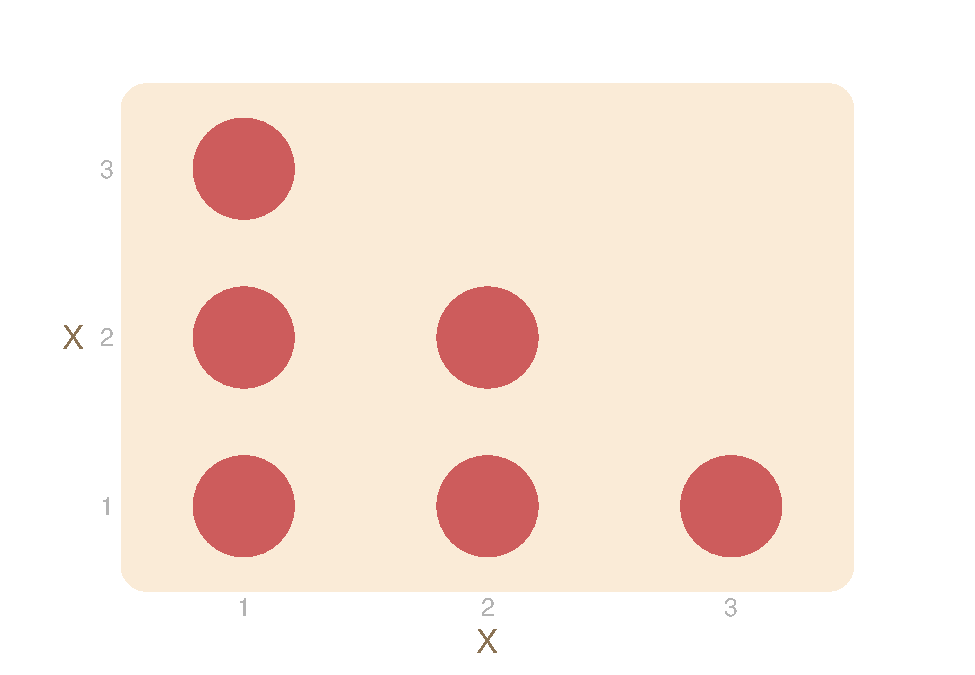
\includegraphics{_main_files/figure-latex/relations-subset-1.pdf}
\caption{\label{fig:relations-subset}Relations as a subset of the Cartesian product on two sets. From the diagram, we see that 1 is less than or equal to every element of y, 2 is less than or equal to 2 and 3, and 3 is less than or equal to 3 only. Note the symmetry between rows and columns - this is due to the fact that we have the same set (\(X\)) on both dimensions.}
\end{figure}

Under some relation \(R\), if two elements \(x, y \in X\) relate, i.e.~if \((x, y) \in R\), we can write this using the infix notation using some infix symbol such as \(\star\): then, if \(x\) and \(y\) relate, we write \(x \star_R y\) or \(x \star y\) (\(R\) implicit). For example, for common relations such as \(=\), \(\leq\), we write \(x = y\) or \(x \leq y\). \(R\) is also sometimes used, e.g.~\(x R y\). If the elements do not relate, i.e.~\((x, y) \not \in R\), we typically do not write this out explicitly.

Relations can have properties. For example, many types of relations are \emph{reflexive}, meaning that \(x \star x\) for all \(x \in X\) (every element relates to itself). Of note, specifying three specific properties allow us to define equivalence relations:

\begin{definition}[Equivalence relation]

A relation \(\sim\) on \(X\) is called an equivalence relation if it is:

\begin{enumerate}
\def\labelenumi{\arabic{enumi}.}
\tightlist
\item
  \emph{Reflexive}: \(x \sim x\) for all \(x \in X\)
\item
  \emph{Symmetric}: \(x \sim y\) if and only if \(y \sim x\) for all \(x, y \in X\)
\item
  \emph{Transitive}: if \(x \sim y\) and \(y \sim z\), then \(x \sim z\)
\end{enumerate}

\end{definition}

Equivalence relations encode the notion that two things are \emph{same-ish}. We can further use them to assign objects in \(X\) to \emph{equivalence classes}, which group equivalent objects together. That is, for some element \(a \in X\), its corresponding equivalence class is:

\[[a] = \{ x \in X : x \sim a \}\]
We can do a lot of things with relations. The next few sections will discuss three important examples: functions, partitions, and preorders.

\hypertarget{functions}{%
\subsection{Functions}\label{functions}}

A function is a special kind of relation that encodes a mapping between two sets. More specifically, let \(S\) be the set of sources (also called the \emph{domain}) and \(T\) be the set of possible targets (also called the \emph{codomain}). Then, we can think of a function as a relation \(F \subseteq S \times T\) of valid source-target pairs \((s, t)\), such that for every \(s \in S\) in there exists a unique \(t \in T\) with \((s, t) \in F\) (see Figure \ref{fig:function-subset}). In other words, every source relates to exactly target, see Figure \ref{fig:function-subset}:

\begin{figure}
\centering
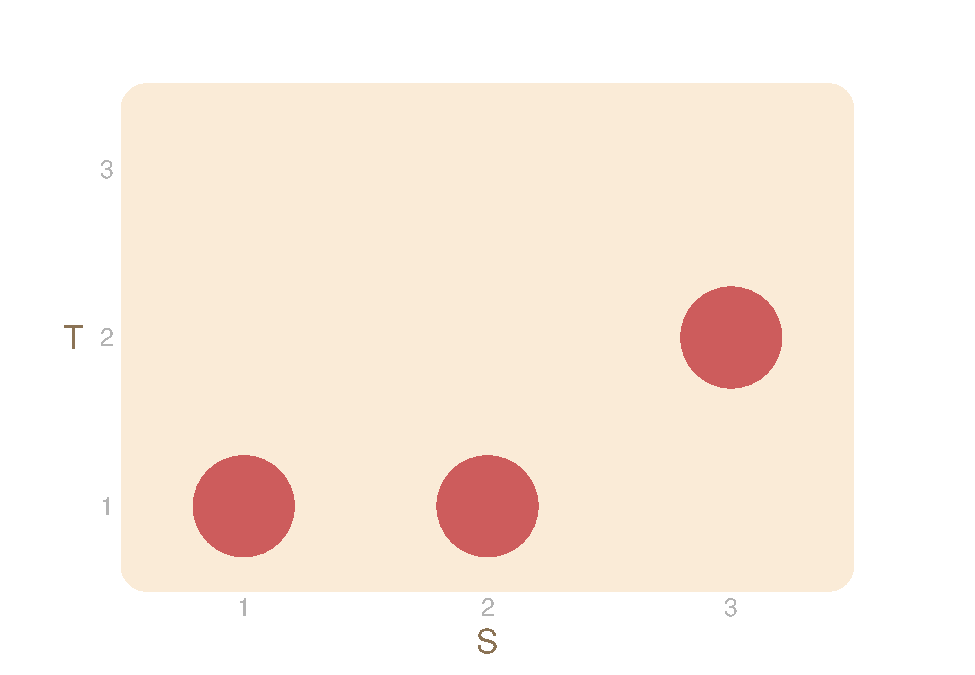
\includegraphics{_main_files/figure-latex/function-subset-1.pdf}
\caption{\label{fig:function-subset}Function as a subset of the Cartesian product on domain (\(S\)) and codomain (\(T\)). The subset \(F \subseteq S \times T\) is shown in red. In words, the function is \(F: \{ 1, 2, 3 \} \to \{ 1, 2, 3 \}\), such that \(F(1) = 1\), \(F(2) = 1\), and \(F(3) = 2\), e.g.~\(f(x) = \lfloor x / 2 \rceil\) (divide by two and round). Note that, for any function, there must be exactly one red dot in each column (each source maps to one and only one target), however, there may be zero or many red dots in any row (some target may not be reachable, or they may be reachable from multiple sources).}
\end{figure}

We can classify functions based on how their domains and codomains map onto each other (see Figure \ref{fig:function-types}). If every target in the function's codomain has a path leading to it from some source, such that no target remains unreachable, then we call it a \emph{surjective} or \emph{onto} function. More formally:

\begin{definition}[Surjectivity]
A function \(f\) is surjective if, for all \(t \in T\), there exists a \(s \in S\) such that \(f(s) = t\).
\end{definition}

Alternatively, if each source in the function's domain leads to a unique target, then we call such a function \emph{injective} or \emph{one-to-one}. That is:

\begin{definition}[Injectivity]
A function is injective if for all \(s_1, s_2 \in S\), if \(f(s_1) = t\) and \(f(s_2) = t\), then \(s_1 = s_2\).
\end{definition}

Finally, if a function is both surjective and injective, meaning that every target can be reached from, and only from, a unique source, then we call such a function \emph{bijective} or a \emph{bijection}.

\begin{definition}[Bijectivity]
A function is a bijection and only if it is both surjective and injective, and if and only if it is invertible.
\end{definition}

\begin{figure}
\centering
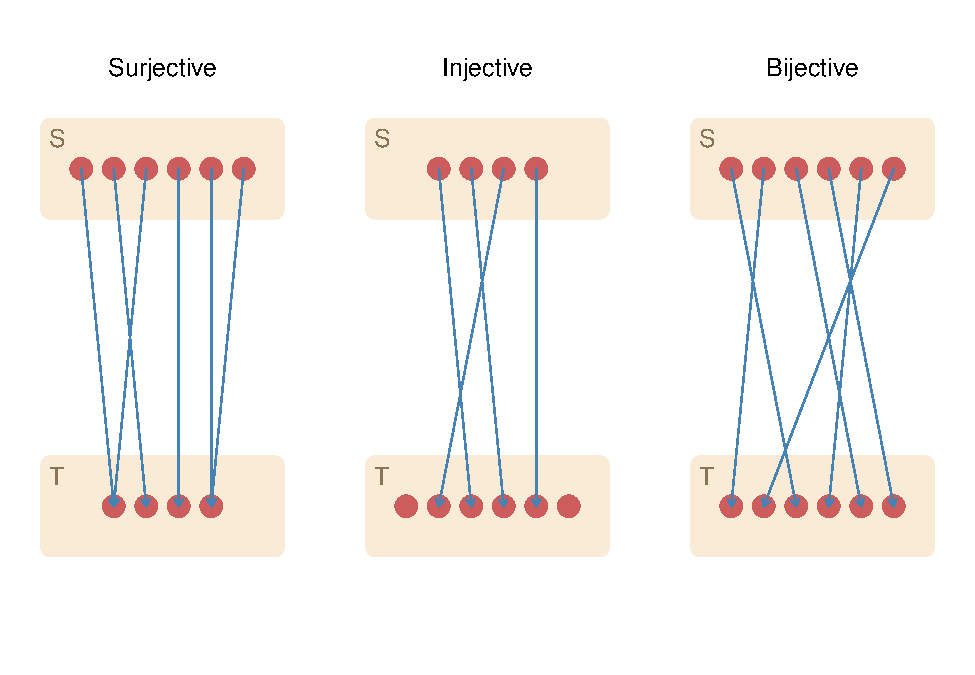
\includegraphics{_main_files/figure-latex/function-types-1.pdf}
\caption{\label{fig:function-types}Types of functions. Left: in a \emph{surjective} function, every target can be reached from some source. Middle: in an \emph{injective} function, every target can only be reached from a unique source. Right: in a \emph{bijection}, every target can be reached from, and only from, a unique source.}
\end{figure}

Bijections are special since they encode the idea of \emph{reversibility} or \emph{lossless transformation}. Any bijective function \(f\) has an associated inverse function \(f^{-1}\) such that \(f^{-1}(f(x)) = x\) and \(f(f^{-1}(a)) = a\) for all \(x\) and \(a\) in the function's domain and codomain, respectively, and we can keep switching back and forth from domain to codomain and back without losing any information. We'll generalize this idea later when we discuss \emph{isomorphisms}.

As an example, suppose I have a group of friends \(f \in F\) that each went to one city \(c \in C\) in Europe during the holiday. I can construct a function \(f: F \to C\) that sends each friend to his or her holiday destination. If every city in \(C\) was visited by at least one friend, then the function is surjective. If each friend went to a different destination, then the function is injective. If both are true - that is, if every city on our list was visited by exactly one friend - then the function is bijective. In that case, we could just as well use the names of cities \(c \in C\) when we speak of friends \(f \in F\) - instead of ``Sam'', we could say ``the person who went to Rome'', and it would be clear who are we talking about.

An important property of functions is that they can be composed. Specifically, if the domain of one function matches the codomain of another, the functions can be composed by piping the output of one into another to form a new function:

\begin{definition}[Function composition]

If we have two functions \(f: X \to Y\) and \(g: Y \to Z\), we can form a new function \(h: X \to Z\) such that:

\[h(x) = g(f(x))\]
We can omit the explicit reference to the variable \(x\) and write the composition in several different ways:

\begin{enumerate}
\def\labelenumi{\arabic{enumi}.}
\tightlist
\item
  \(h = g \circ f\) (read: ``apply \(g\) after \(f\)'')
\item
  \(h = gf\) (same as above)
\item
  \(h = f ⨾ g\) (read ``apply \(f\) then \(g\)'')
\end{enumerate}

\end{definition}

I will use the bracket notation (\(h(x) = g(f(x))\)) when explicitly referring to the variable, and the postfix/fat semicolon notation (\(h = f ⨾ g\)) otherwise.

There are other things we can do with functions. For example, given a subset of sources, we can ask about the \emph{image} - the set of targets we can reach from those sources:

\begin{definition}[Image]
For some subset \(S_i \subseteq S\), its image under \(f\) is defined as \(f_!(S_i) = \{ f(s) \in T \lvert s \in S_i \}\).
\end{definition}

Likewise, given a subset of targets, we can ask about the \emph{pre-image} - the set of sources that could have produced those targets. That is:

\begin{definition}[Pre-image]
For some subset \(T_i \subseteq T\), its pre-image under \(f\) is defined as \(f^*(T_i) = \{ s \in S \lvert f(s) \in T_i \}\).
\end{definition}

An important fact to note is that, although the pre-image \(f^*\) is also sometimes called ``inverse image'', it is \emph{not} the inverse of the image \(f_!\) for most functions (unless they are bijections). That is, by applying the pre-image after image or vice versa, we cannot expect to come up with the same set as we started with. Specifically, if we have a non-injective function and apply the pre-image after the image, we may come up with \emph{more} sources that we started with, \(S_i \subseteq f^*(f_!(S_i))\) (equality if injective), and similarly, if we have a non-surjective function and apply the image after the pre-image, we might end up with \emph{fewer} targets than we started with, \(f_!(f^*(T_i)) \subseteq T_i\) (again, equality if surjective).

As an example, suppose again I have the function \(f\) which maps each friend to a holiday destination. The image of that function, \(f_!\), maps a set of friends to the set of all cities that at least one of them went to, and similarly, the pre-image, \(f^*\), maps a set of cities to the set of friends that went to them.\\
Now, suppose that Sam and Dominic went to Rome, and I ask:

\begin{quote}
\emph{``who went to {[}the city that Sam went to{]}?''}
\end{quote}

I will get both Sam and Dominic back, since:

\[f^*(f_!(\{ Sam \})) = f^*(\{ Rome \}) = \{ Sam, Dominic \}\]

That is, I will get back Sam and Dominic \emph{even though I had initially only asked about Sam}. Similarly, if no friends had visited Paris and I ask:

\begin{quote}
\emph{``what are the cities that {[}people who went to Paris or Rome{]} went to?''}
\end{quote}

then I will get Rome only, since

\[f_!(f^*(\{Paris, Rome \})) = f_!(\{ Sam, Dominic \}) = \{ Rome \}\]

This weird relationship between the the image and the pre-image is due to the fact that the image is actually something called \emph{left adjoint} (\protect\hyperlink{ref-baez2023}{Baez 2023}; \protect\hyperlink{ref-fong2019}{Fong and Spivak 2019}). Adjoints can be thought of as the ``best approximate answer to a problem that has no solution'' (no inverse, \protect\hyperlink{ref-baez2023}{Baez 2023}), and they come in pairs - a left and a right adjoint - with the left adjoint being more permissive or ``liberal'' and the right adjoint being more strict or ``conservative'' (\protect\hyperlink{ref-baez2023}{Baez 2023}).

Proper treatment of adjoint is beyond the scope of this thesis, however.

\hypertarget{partitions}{%
\subsection{Partitions}\label{partitions}}

One useful thing we can construct with functions (or equivalently, relations) are partitions. Partitions encode the idea of splitting elements of some some into distinct groups.

\begin{definition}[Function definition of a partition]
Given some set \(X\), a set of part labels \(P\), and a surjective function \(f: X \to P\), we can partition \(A\) by assigning every element \(x \in X\) a part label \(p \in P\), by simply applying the function: \(f(x) = p\).
\end{definition}

Above we used a function to define a partition, however, we can achieve the same with a relations, specifically equivalence classes. By taking any part label \(p \in P\), we can recover the corresponding subset of \(X\) by pulling out its pre-image: \(f^*(\{p\}) = X_p \subseteq X\). We can then define a partition without reference to \(f\):

\begin{definition}[Equivalence class definition of a partition]
A partition of \(A\) consists of a set of part labels \(P\), such that, for all \(p \in P\), there is a non-empty subset \(A_p \subseteq A\) which forms an equivalence class on \(A\) and:

\[X = \bigcup_{p \in P} X_p \qquad \text{and} \qquad \text{if } p \neq q, \text{ then } X_p \cap X_q = \varnothing\]
I.e. the parts \(X_p\) jointly cover the entirety of \(X\) and parts cannot share any elements.
\end{definition}

We can rank partitions by their coarseness. That is, for any set \(X\), the coarsest partition is one with only one part label \(P = \{ 1 \}\), such that each element of \(X\) gets assigned \(1\) as label. Conversely, the finest partition is one where each element gets assigned its own unique part label, such that \(\lvert X \lvert = \lvert P \lvert\).

Given two partitions, we can form a finer (or at least as fine) partition by taking their intersection, i.e.~by taking the set of all unique pairs of labels that co-occur for any \(x \in X\) as the new part labels. For example, suppose \(X = \{ 1, 2, 3 \}\) and partition 1 assigns part labels:

\[p_1(x) = \begin{cases} 
a & \text{if } x = 1 \text{ or } x = 2 \\
b & \text{if } x = 3
\end{cases}\]

and partition 2 assigns part labels the following way:

\[
p_2(a) = \begin{cases}
s & \text{if } x = 1 \\
t & \text{if } x = 2 \text{ or } x = 3
\end{cases}
\]

Then the intersection partition will have the following part labels \(P_3 = \{ (a, s), (a, t), (b, t) \}\) such that:

\[
p_3(a) = \begin{cases}
(a, s) & \text{if } x = 1 \\
(b, s) & \text{if } x = 2 \\ 
(b, t) & \text{if } x = 3
\end{cases}
\]

\hypertarget{preorders}{%
\subsection{Preorders}\label{preorders}}

\begin{definition}[Preorder]

A preorder is a set \(X\) equipped with a binary relation \(\leq\) that conforms to two simple properties:

\begin{enumerate}
\def\labelenumi{\arabic{enumi}.}
\tightlist
\item
  \emph{Reflexivity}: \(x \leq x\) for all \(x \in X\)
\item
  \emph{Transitivity}: if \(x \leq y\) and \(y \leq z\), then \(x \leq z\), for all \(x, y, z \in X\)
\end{enumerate}

\end{definition}

Simply speaking, this means that between any two elements in \(X\), there either is a relation and the elements relate (one element is somehow ``less than or equal'' to the other), or the two elements do not relate.

An example of a preorder is the family tree, with the underlying set being the set of family members: \(X = \{ \textbf{daughter}, \textbf{son}, \textbf{mother}, \textbf{father}, \textbf{grandmother}, ... \}\) and the binary relation being ancestry or familial relation. Thus, for example, \(\textbf{daughter} \leq \textbf{father}\), since the daughter is related to the father, and \(\textbf{father} \leq \textbf{father}\), since a person is related to themselves. However, there is no relation (\(\leq\)) between \(\textbf{father}\) and \(\textbf{mother}\) since they are not related. Finally, since \(\textbf{daughter} \leq \textbf{father}\) and \(\textbf{father} \leq \textbf{grandmother}\), then, by reflexivity, \(\textbf{daughter} \leq \textbf{grandmother}\).

We can further restrict preorders by imposing additional properties, such as:

\begin{enumerate}
\def\labelenumi{\arabic{enumi}.}
\setcounter{enumi}{2}
\tightlist
\item
  If \(x \leq y\) and \(y \leq x\), then \(x = y\) (anti-symmetry)
\item
  Either \(x \leq y\) or \(y \leq x\) (comparability)
\end{enumerate}

If a preorder conforms to 3., we speak of a partially ordered set or \emph{poset}. If it conforms to both 3. and 4., then it is a \emph{total order}.

\hypertarget{monoids}{%
\section{Monoids}\label{monoids}}

A monoid is a tuple \((M, e, \otimes)\) consisting of:

\begin{enumerate}
\def\labelenumi{\alph{enumi}.}
\tightlist
\item
  A set of objects \(M\)
\item
  A neutral element \(e\) called the \emph{monoidal unit}
\item
  A binary function \(\otimes: M \times M \to M\) called the \emph{monoidal product}
\end{enumerate}

Such that:

\begin{enumerate}
\def\labelenumi{\arabic{enumi}.}
\tightlist
\item
  \(m \otimes e = e \otimes m = m\) for all \(m \in M\) (unitality)
\item
  \(m_1 \otimes (m_2 \otimes m_3) = (m_1 \otimes m_2) \otimes m_3 = m_1 \otimes m_2 \otimes m_3\) for all \(m_1, m_2, m_3 \in M\) (associativity)
\end{enumerate}

In simple terms, monoids encapsulate the idea that \emph{the whole is exactly the ``sum'' of its parts} (where ``sum'' can be replaced by the monoidal product). Specifically, we have some elements and a way to combine them, and when we combine the same elements, no matter where we put the brackets we always get the same result (i.e.~something like ``the order does not matter'', although that is not precisely right, more on that later). Finally, we have some neutral element that when combined with an element yields back the same element.

For example, take summation on natural numbers, \((\mathbb{N}, 0, +)\):

\[1 + 0 = 0 + 1 = 1 \qquad \text{(unitality)}\]
\[1 + (2 + 3) = (1 + 2) + 3 = 1 + 2 + 3 \qquad \text{(associativity)}\]

Likewise, products of real numbers \((\mathbb{R}, 1, \times)\) are also a monoid, and so is multiplication of \(n \times n\) square matrices \((\mathbf{M}_{n \in \mathbb{Z}}, \mathbf{I}, \cdot)\), where \(\mathbf{I}\) is the identity matrix and \(\cdot\) stands for an infix operator that is usually omitted. As a counterexample, exponentiation does not meet the definition of a monoid, since it is not associative: \(x^{(y^z)} \neq (x^y)^z\).

We may want to impose further restrictions on monoids, for example:

\begin{enumerate}
\def\labelenumi{\arabic{enumi}.}
\setcounter{enumi}{2}
\tightlist
\item
  \(m_1 \otimes m_2 = m_2 \otimes m_1\) for all \(m_1, m_2 \in M\) (commutativity)
\end{enumerate}

Both commutativity and associativity can both be viewed as a kind of ``order does not matter'' rule, however, they are fundamentally different. Let's imagine our set of objects consists of three wires of different colours \(\{ \textbf{red}, \textbf{green}, \textbf{blue} \}\) and the monoidal product consists of connecting wires. Let's also imagine that the \(\textbf{red}\) wire is connected to a power source and the \(\textbf{blue}\) wire is connected to a lightbulb, and the blue wire amplifies the current from the power source such that it is enough to power the light bulb. To turn on the lightbulb, we need to connect \(\textbf{red} \to \textbf{green}\) and \(\textbf{green} \to \textbf{blue}\). The time order in which we connect the three wires does not matter: we can connect \(\textbf{green} \to \textbf{blue}\) first and \(\textbf{red} \to \textbf{green}\) second or vice versa, either way we get the same result (lightbulb turns on). However, the spatial order in which we connect the wires \emph{does} matter: if we connect \(\textbf{red} \to \textbf{blue}\), then the current will not be enough to power the lightbulb. Hence, the operation is associative (temporal order does not matter) but not commutative (spatial order does matter).

If \(M\) is a preorder, another restriction we may want to impose is that the monoidal product is strictly increasing:

\begin{enumerate}
\def\labelenumi{\arabic{enumi}.}
\setcounter{enumi}{3}
\tightlist
\item
  \(m_1 \leq m_1 \otimes m_2\) and \(m_2 \leq m_1 \otimes m_2\) for all \(m_1, m_2 \in M\) (monotonicity)
\end{enumerate}

This means that when we combine two things, we get back something that's at least as big as the bigger of the two things. Summation of natural numbers \((\mathbb{N}, 0, +)\) again works, but for example summation of integers \((\mathbb{Z}, 0, +)\) or multiplication of reals \((\mathbb{R}, 1, \times)\) does not.

\hypertarget{data-visualization-systems}{%
\section{Data Visualization Systems}\label{data-visualization-systems}}

\hypertarget{scales}{%
\subsection{Scales}\label{scales}}

Every data visualization system needs some way of translating abstract data values into concrete graphical attributes such as position, size, or colour. Given the ubiquitous need for scales, one might expect them to be a ``solved issue'', within the relevant literature. However, this is far from the truth. Specifically, the issues of scales and measurement present are still being grappled with the areas of mathematics and philosophy of science to this day (for a gentle yet thorough introduction, see \protect\hyperlink{ref-tal2015}{Tal 2015}).

Scales are another area of data visualization in which there has been considerable debate, with many terms being overloaded and relating to concepts from different fields. This is due to the fact that the issue of how to compare, rank, and translate values has a long and complicated history. In particular, the issue of measurement has been hotly debated in the field of psychometrics and mathematical psychology, leading to the development of the \emph{theory of measurement} (which has some overlap with, but is not the same as, \emph{measurement theory} in mathematics).

One paper that has been key to the debate around scales and measurement has been the seminal work of Stevens (\protect\hyperlink{ref-stevens1946}{1946}). In this paper, Stevens defined a \emph{scale} as a method of assigning numbers to values, allowing for various kinds of comparisons. Further, by considering transformations which preserve the comparisons, Stevens identified 4 types of scales: \emph{nominal}, \emph{ordinal}, \emph{interval}, and \emph{ratio} (see also \protect\hyperlink{ref-michell1986}{Michell 1986}; \protect\hyperlink{ref-velleman1993}{Velleman and Wilkinson 1993}).

\begin{table}

\caption{\label{tab:scales}Types of scales identified by Stevens (1946)}
\centering
\begin{tabular}[t]{l|l|l|l}
\hline
Scale & Structure & Comparison & Valid transformations\\
\hline
Nominal & Equivalence relation & Are \$x\$ and \$y\$ the same? & \$x' = f(x)\$ where \$f\$ is a bijection\\
\hline
Ordinal & Total order & Is \$x\$ is greater than \$y\$? & \$x' = f(x)\$ where \$f\$ is a monotonically increasing bijection\\
\hline
Interval & Lebesque measure & Is the distance from \$x\$ to \$y\$ the same as from \$a\$ to \$b\$? & \$x' = ax + b\$\\
\hline
Ratio &  & How many times is \$x\$ greater than \$y\$? & \$x' = ax\$\\
\hline
\end{tabular}
\end{table}

Table \ref{tab:scales} shows a loose reproduction of Table 1 from Stevens (\protect\hyperlink{ref-stevens1946}{1946}). Note that the family of valid transformations gets smaller in each row, meaning that the scales carry more information (\protect\hyperlink{ref-velleman1993}{Velleman and Wilkinson 1993}). Let's discuss the scales individually.

\hypertarget{nominal-scales}{%
\paragraph{Nominal scales}\label{nominal-scales}}

\emph{Nominal} scales correspond to equivalence relations. An equivalence relation is a binary relation \(\sim\) on some set \(X\) which, for all \(x, y, z \in X\), has the following properties:

\begin{itemize}
\tightlist
\item
  \emph{Reflexivity}: \(x \sim x\)
\item
  \emph{Symmetry}: \(x \sim y \text{ if and only if } y \sim x\)
\item
  \emph{Transitivity}: \(x \sim y \text{ and } y \sim z \text{ then } x \sim z\)
\end{itemize}

Intuitively, we can think of the numbers on a nominal scale as ``labels'', and the only question which we can ask a nominal scale is whether two labels are the same or different. A such, examples of variables with nominal scale include variables of which we typically think of as categorical, such as color, species, or political party. It does not make sense to say ``blue is \emph{more} than green'' or ``cat is \emph{more} than dog'' without specifying some other axis along which we compare. It does make sense, however, to say ``Daisy and Molly are the same species of animal (cat)'' or ``these two glasses are of different colors''.

The only transformations which are permissible for nominal scales are permutations (\protect\hyperlink{ref-stevens1946}{Stevens 1946}). For example, if we use the numbers \(\{ 1, 2, 3 \}\) to represent the species \(S = \{ \text{cat}, \text{dog}, \text{hamster} \}\), respectively, we can assign the numbers in any order we want and the properties of the scale are preserved.

It is arguable whether any nominal quantities exist in and of themselves or whether they only ever exists as abstract social constructions over underlying continuous reality. Color is a discretization of the visible light spectrum (frequency of electromagnetic radiation), and the pre-Darwinian concept of a species is likewise an abstraction over continuously varying distribution of genes (although there have been some attempts to ground the definition of a discrete species in the theory of genetics, e.g.~as a population of individuals which can produce viable offsprings, see \protect\hyperlink{ref-mayr1999}{Mayr 1999}). Further, even many subjective concepts which are typically described as discrete such as emotions may be abstractions over underlying continuous phenomena (\protect\hyperlink{ref-barrett2013}{Barrett 2013}).

However, even if nominal quantities are entirely socially constructed, this does not mean they are arbitrary or useless. SEARLE

\hypertarget{ordinal-scales}{%
\paragraph{Ordinal scales}\label{ordinal-scales}}

\emph{Ordinal} scales correspond to total orders. A total order is a relation \(\leq\) on \(X\) which, for all \(x, y, z \in X\), has the following properties:

\begin{enumerate}
\def\labelenumi{\arabic{enumi})}
\tightlist
\item
  \emph{Reflexivity}: \(x \leq x\)
\item
  \emph{Antisymmetry}: \(\text{if } x \leq y \leq x \text{ then } x = y\)
\item
  \emph{Transitivity}: \(x \leq y \text{ and } y \leq z \text{ then } x \leq z\)
\item
  \emph{Totality} or \emph{comparability} or \emph{strong connectedness}: \(\text{for all } x, y, \text{ either } x \leq y \text{ or } y \leq x\)
\end{enumerate}

Examples of total orders include the usual ordering \(\leq\) on natural numbers \(\mathbb{N}\): \(1 \leq 2 \leq 3 \leq \ldots\) or the alphabetical order on letters: \(A \leq B \leq C \ldots \leq Z\).

As total orders, ordinal scales allow us to rank quantities. A good example of an ordinal variable is placement in a race or competition. If Emma and Charlotte ran a marathon, and Emma placed 2nd and Charlotte 3rd, we can say that Charlotte ran finished the race earlier than Emma. However, we do not know whether she crossed the finish line 15 minutes or 2 hours earlier, or whether or not her average pace was less than half of that of Emma.

Some authors have related ordinal scales to \emph{weak orders} (see \protect\hyperlink{ref-michell1986}{Michell 1986}). Weak orders (also known as \emph{total preorders}, see \protect\hyperlink{ref-nlab2024d}{nLab 2024a}) generalize total orders by allowing for ties (properties 2. and 4. above do not need hold). While this could seem desirable, I opted to relate ordinal scales to total orders here instead, since there is currently some ambiguity in the literature in the way the term \emph{weak order} is being used (see e.g. \protect\hyperlink{ref-nlab2024a}{nLab 2024b}, \protect\hyperlink{ref-nlab2024b}{2024c}; \protect\hyperlink{ref-stackexchange2024}{Abrams 2024}), and, for practical data analysis, the distinction is fairly inconsequential. For instance, in the marathon example above, if Emma and Charlotte both placed second, after Lucy and before Lily, we could frame the outcome of the race as the following weak order on the set \(M\) of marathoners: \(\text{Lucy} \leq \text{Emma, Charlotte} \leq \text{Lily} \leq ...\). However, the underlying set of ranks \(R \subset \mathbb{N}\) still retains a total ordering: \(1 \leq 2 \leq 3 \leq \ldots\) and we can specify a surjective monotonically increasing function \(r: M \to R\) which maps each marathoner to her rank. Clearly, we can map any weak order to a total order by applying a functor which enforces anti-symmetry in this way (\protect\hyperlink{ref-fong2019}{Fong and Spivak 2019}; \protect\hyperlink{ref-nlab2024d}{nLab 2024a}).

The only transformations which are permissible for ordinal scales are those which preserve order, that is, monotonic increasing transformations (\protect\hyperlink{ref-stevens1946}{Stevens 1946}; \protect\hyperlink{ref-michell1986}{Michell 1986}). For example, transforming our set of ranks \(R\) by taking the log or square root of each rank leaves the order relations between them unchanged.

\hypertarget{interval-scales}{%
\paragraph{Interval scales}\label{interval-scales}}

\emph{Interval} scales.

Interval scales allow us to identify a distance between two points. However, they do not have a natural ``zero point'' or intercept. As such we cannot use them to determine the ratio between two quantities. Examples of interval scales include the calendar date and geographical position. It does not make sense to say that the year 1000 CE is ``twice'' that of 500 CE, since the birth of Jesus Christ is (one's personal religious beliefs aside) an arbitrary zero point: we could set the point 0 CE to any other event, such as the founding of Athens or the release of Taylor Swift's first album, and the ratios would be altered. Likewise, it does not make sense to say that 90° longitude is ``three times'' that of 30° longitude: the location of the prime meridian is also the product of arbitrary historical cirumstances.

\hypertarget{ratio-scales}{%
\subparagraph{Ratio scales}\label{ratio-scales}}

Unlike interval scales, ratio scale have a well-defined natural zero point. For example,

\hypertarget{criticism-of-on-the-theory-of-scales-of-measurement}{%
\paragraph{Criticism of On the Theory of Scales of Measurement}\label{criticism-of-on-the-theory-of-scales-of-measurement}}

In the original paper, Stevens had also made the claim that the type of scale determined which statistical tests and summaries were ``permissible'' for the data. For example, according to Stevens, while mean is an appropriate summary of an interval scale (since expectation is linear), it would not be a permissible summary of ordinal data. This claim was later disputed by researchers

\hypertarget{design}{%
\chapter{Design}\label{design}}

Placeholder

\hypertarget{factors}{%
\subsection{Factors}\label{factors}}

\hypertarget{product-factors}{%
\subsubsection{Product factors}\label{product-factors}}

\hypertarget{reducers}{%
\subsection{Reducers}\label{reducers}}

\hypertarget{scales-1}{%
\subsection{Scales}\label{scales-1}}

\hypertarget{expanses}{%
\subsection{Expanses}\label{expanses}}

\hypertarget{zero-and-one}{%
\subsubsection{Zero and One}\label{zero-and-one}}

\hypertarget{expanse-interface}{%
\subsubsection{Expanse Interface}\label{expanse-interface}}

\hypertarget{continuous-expanses}{%
\subsubsection{Continuous Expanses}\label{continuous-expanses}}

\hypertarget{linearity}{%
\paragraph{Linearity}\label{linearity}}

\hypertarget{transformations}{%
\paragraph{Transformations}\label{transformations}}

\hypertarget{references}{%
\chapter{References}\label{references}}

\hypertarget{refs}{}
\begin{CSLReferences}{1}{0}
\leavevmode\vadjust pre{\hypertarget{ref-stackexchange2024}{}}%
Abrams, Dave. 2024. {``Total Weak Order Vs Total Order.''} \emph{Mathematics Stack Exchange}. \url{https://math.stackexchange.com/questions/3793222/total-weak-order-vs-total-order}.

\leavevmode\vadjust pre{\hypertarget{ref-baez2023}{}}%
Baez, John. 2023. {``{Applied Category Theory Course}.''} \url{https://math.ucr.edu/home/baez/act_course}.

\leavevmode\vadjust pre{\hypertarget{ref-barrett2013}{}}%
Barrett, Lisa Feldman. 2013. {``Psychological Construction: The Darwinian Approach to the Science of Emotion.''} \emph{Emotion Review} 5 (4): 379--89.

\leavevmode\vadjust pre{\hypertarget{ref-beckmann1995}{}}%
Beckmann, Peter E. 1995. {``On the Problem of Visualizing Point Distributions in High Dimensional Spaces.''} \emph{Computers \& Graphics} 19 (4): 617--29.

\leavevmode\vadjust pre{\hypertarget{ref-fong2019}{}}%
Fong, Brendan, and David I Spivak. 2019. \emph{An Invitation to Applied Category Theory: Seven Sketches in Compositionality}. Cambridge University Press.

\leavevmode\vadjust pre{\hypertarget{ref-kindlmann2014}{}}%
Kindlmann, Gordon, and Carlos Scheidegger. 2014. {``An Algebraic Process for Visualization Design.''} \emph{IEEE Transactions on Visualization and Computer Graphics} 20 (12): 2181--90.

\leavevmode\vadjust pre{\hypertarget{ref-lawvere2009}{}}%
Lawvere, F William, and Stephen H Schanuel. 2009. \emph{Conceptual Mathematics: A First Introduction to Categories}. Cambridge University Press.

\leavevmode\vadjust pre{\hypertarget{ref-mayr1999}{}}%
Mayr, Ernst. 1999. \emph{Systematics and the Origin of Species, from the Viewpoint of a Zoologist}. Harvard University Press.

\leavevmode\vadjust pre{\hypertarget{ref-michell1986}{}}%
Michell, Joel. 1986. {``Measurement Scales and Statistics: A Clash of Paradigms.''} \emph{Psychological Bulletin} 100 (3): 398.

\leavevmode\vadjust pre{\hypertarget{ref-milewski2018}{}}%
Milewski, Bartosz. 2018. \emph{Category Theory for Programmers}. Blurb.

\leavevmode\vadjust pre{\hypertarget{ref-nlab2024d}{}}%
nLab. 2024a. {``Posetal Reflection in nLab.''} \url{https://ncatlab.org/nlab/show/posetal+reflection}.

\leavevmode\vadjust pre{\hypertarget{ref-nlab2024a}{}}%
---------. 2024b. {``Strict Weak Order in nLab.''} \url{https://ncatlab.org/nlab/show/strict+weak+order}.

\leavevmode\vadjust pre{\hypertarget{ref-nlab2024b}{}}%
---------. 2024c. {``Weak Order in nLab.''} \url{https://ncatlab.org/nlab/show/weak+order}.

\leavevmode\vadjust pre{\hypertarget{ref-petricek2021}{}}%
Petricek, Tomas. 2021. {``Composable Data Visualizations.''} \emph{Journal of Functional Programming} 31: e13.

\leavevmode\vadjust pre{\hypertarget{ref-smeltzer2018}{}}%
Smeltzer, Karl, and Martin Erwig. 2018. {``A Domain-Specific Language for Exploratory Data Visualization.''} In \emph{Proceedings of the 17th ACM SIGPLAN International Conference on Generative Programming: Concepts and Experiences}, 1--13.

\leavevmode\vadjust pre{\hypertarget{ref-smeltzer2014}{}}%
Smeltzer, Karl, Martin Erwig, and Ronald Metoyer. 2014. {``A Transformational Approach to Data Visualization.''} In \emph{Proceedings of the 2014 International Conference on Generative Programming: Concepts and Experiences}, 53--62.

\leavevmode\vadjust pre{\hypertarget{ref-stevens1946}{}}%
Stevens, Stanley Smith. 1946. {``On the Theory of Scales of Measurement.''} \emph{Science} 103 (2684): 677--80.

\leavevmode\vadjust pre{\hypertarget{ref-tal2015}{}}%
Tal, Eran. 2015. {``Measurement in Science.''}

\leavevmode\vadjust pre{\hypertarget{ref-velleman1993}{}}%
Velleman, Paul F, and Leland Wilkinson. 1993. {``Nominal, Ordinal, Interval, and Ratio Typologies Are Misleading.''} \emph{The American Statistician} 47 (1): 65--72.

\leavevmode\vadjust pre{\hypertarget{ref-yorgey2012}{}}%
Yorgey, Brent A. 2012. {``Monoids: Theme and Variations (Functional Pearl).''} \emph{ACM SIGPLAN Notices} 47 (12): 105--16.

\end{CSLReferences}

\end{document}
